\section{Iterative word-serial}\label{sec:wordserial}

This architecture is the direct implementation of the \cordic{} equations.

The Cartesian coordinates are loaded into the registers, passing through a
multiplexer that will be used in the following stages to store the partial
results of the algorithm.

At each clock cycle an iteration is performed, so to have the final result
\(n+1\) clock cycles are needed (one more for loading the values into the
registers). The throughput of the system is one result every \(n+1\) clock
cycles. The sign control logic can be implemented using the \textit{MSB} of
\(y_{i+1}\)

\figref{fig:wordserial} shows the block diagram for this architecture.

\begin{figure}[hb]
	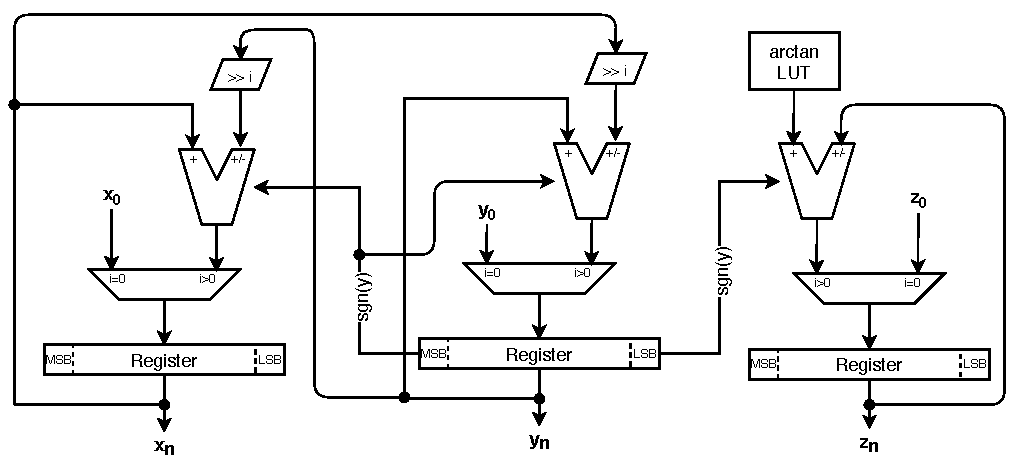
\includegraphics[width=\textwidth]{wordserial}
	\caption{Block diagram of the iterative word-serial architecture.}\label{fig:wordserial}
\end{figure}
